%!TEX root = ../main.tex

\begin{figure}
\newcommand{\xdisposition}{0}
\newcommand{\ydisposition}{0}
\newcommand{\xtstep}{0.75}
\newcommand{\ytstep}{0.7}
\newcommand{\ybias}{-0.3 }
\newcommand{\xstep}{2.5}
\newcommand{\ystep}{-0.475}
\newcommand{\xtscale}{0.8}

\def \numevents{15.5}

\newcommand{\eventA}[4]{
\node[event, draw=black, fill=white] (A#1) at (#1*\xstep, #2*\ystep) {\footnotesize $#2(x_{#3})$};
%\node[] at (0*\xstep-\xtstep, {#1*\ystep}) {\small $#2(x_{#3})$};
}

\scalebox{0.95}{
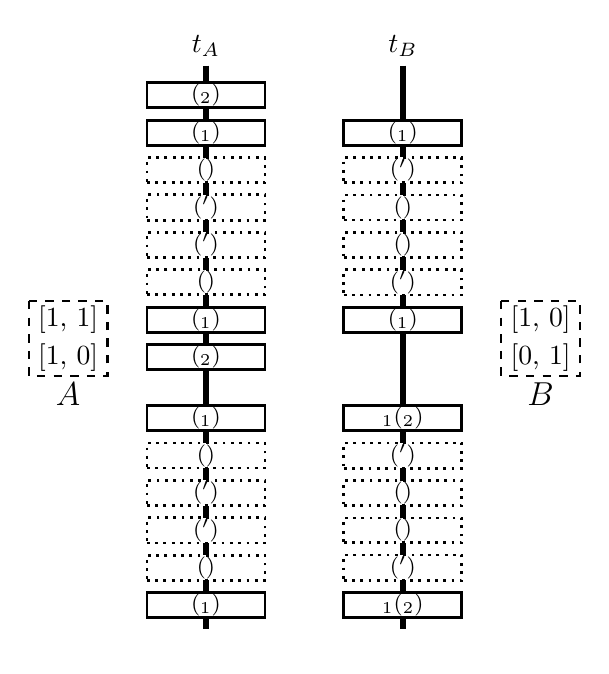
\begin{tikzpicture}[thick,
pre/.style={<-,shorten >= 2pt, shorten <=2pt, very thick},
post/.style={->,shorten >= 3pt, shorten <=3pt,   thick},
seqtrace/.style={line width=2},
und/.style={very thick, draw=gray},
event/.style={rectangle, minimum height=0.8mm, minimum width=15mm,  line width=1pt, inner sep=0.5,},
virt/.style={circle,draw=black!50,fill=black!20, opacity=0}]
\footnotesize


\draw[dashed] (-0.9*\xstep,6.5*\ystep) rectangle (-0.5*\xstep,8.5*\ystep);
\node (A1) at (-0.7*\xstep,7*\ystep) {\normalsize [1, 1]};
\node (A2) at (-0.7*\xstep,8*\ystep) {\normalsize [1, 0]};
\node (A) at (-0.7*\xstep,9*\ystep) {\large  $A$};

\draw[dashed] (1.5*\xstep,6.5*\ystep) rectangle (1.9*\xstep,8.5*\ystep);
\node (B1) at (1.7*\xstep,7*\ystep) {\normalsize [1, 0]};
\node (B2) at (1.7*\xstep,8*\ystep) {\normalsize [0, 1]};
\node (B) at (1.7*\xstep,9*\ystep) {\large  $B$};


\node[] (S11) at (0*\xstep,0.15) {\normalsize $t_A$};
\node[] (S12) at (0*\xstep,\numevents * \ystep) {};
\node[] (S21) at (1*\xstep,0.15) {\normalsize $t_B$};
\node[] (S22) at (1*\xstep,\numevents * \ystep) {};

\draw[seqtrace] (S11) to (S12);
\draw[seqtrace] (S21) to (S22);


\node[event, draw=black, fill=white] (11) at (0*\xstep, 1*\ystep + 0*\ybias) {$\acq(\lk_2)$};
\node[event, draw=black, fill=white] (12) at (0*\xstep, 2*\ystep + 0*\ybias) {$\acq(\lk_1)$};
\node[event, draw=black, fill=white, dotted] (13) at (0*\xstep, 3*\ystep + 0*\ybias) {$\acq(\lk)$};
\node[event, draw=black, fill=white, dotted] (14) at (0*\xstep, 4*\ystep + 0*\ybias) {$\acq(\lk')$};
\node[event, draw=black, fill=white, dotted] (15) at (0*\xstep, 5*\ystep + 0*\ybias) {$\rel(\lk')$};
\node[event, draw=black, fill=white, dotted] (16) at (0*\xstep, 6*\ystep + 0*\ybias) {$\rel(\lk)$};
\node[event, draw=black, fill=white] (17) at (0*\xstep, 7*\ystep + 0*\ybias) {$\rel(\lk_1)$};
\node[event, draw=black, fill=white] (18) at (0*\xstep, 8*\ystep + 0*\ybias) {$\rel(\lk_2)$};

\node[event, draw=black, fill=white] (19) at (0*\xstep, 9*\ystep + 1*\ybias) {$\acq(\lk_1)$};
\node[event, draw=black, fill=white, dotted] (110) at (0*\xstep, 10*\ystep + 1*\ybias) {$\acq(\lk)$};
\node[event, draw=black, fill=white, dotted] (111) at (0*\xstep, 11*\ystep + 1*\ybias) {$\acq(\lk')$};
\node[event, draw=black, fill=white, dotted] (112) at (0*\xstep, 12*\ystep + 1*\ybias) {$\rel(\lk')$};
\node[event, draw=black, fill=white, dotted] (113) at (0*\xstep, 13*\ystep + 1*\ybias) {$\rel(\lk)$};
\node[event, draw=black, fill=white] (114) at (0*\xstep, 14*\ystep + 1*\ybias) {$\rel(\lk_1)$};

%%%%%%%%%%%%%%%%

\node[event, draw=black, fill=white] (21) at (1*\xstep, 2*\ystep + 0*\ybias) {$\acq(\lk_1)$};
\node[event, draw=black, fill=white, dotted] (22) at (1*\xstep, 3*\ystep + 0*\ybias) {$\acq(\lk')$};
\node[event, draw=black, fill=white, dotted] (23) at (1*\xstep, 4*\ystep + 0*\ybias) {$\acq(\lk)$};
\node[event, draw=black, fill=white, dotted] (24) at (1*\xstep, 5*\ystep + 0*\ybias) {$\rel(\lk)$};
\node[event, draw=black, fill=white, dotted] (25) at (1*\xstep, 6*\ystep + 0*\ybias) {$\rel(\lk')$};
\node[event, draw=black, fill=white] (26) at (1*\xstep, 7*\ystep + 0*\ybias) {$\rel(\lk_1)$};

\node[event, draw=black, fill=white] (27) at (1*\xstep, 9*\ystep + 1*\ybias) {$\acq_1(\lk_2)$};
\node[event, draw=black, fill=white, dotted] (28) at (1*\xstep, 10*\ystep + 1*\ybias) {$\acq(\lk')$};
\node[event, draw=black, fill=white, dotted] (29) at (1*\xstep, 11*\ystep + 1*\ybias) {$\acq(\lk)$};
\node[event, draw=black, fill=white, dotted] (210) at (1*\xstep, 12*\ystep + 1*\ybias) {$\rel(\lk)$};
\node[event, draw=black, fill=white, dotted] (211) at (1*\xstep, 13*\ystep + 1*\ybias) {$\rel(\lk')$};
\node[event, draw=black, fill=white] (212) at (1*\xstep, 14*\ystep + 1*\ybias) {$\rel_1(\lk_2)$};


\end{tikzpicture}
}
\caption{
Reduction for OV-hardness proof from an instance of size $n = 2$ and $d = 2$.
}
\figlabel{ov-hardness}
\end{figure}